\documentclass[10pt,twocolumn,letterpaper]{article}

\usepackage[utf8]{inputenc}
\usepackage[T1]{fontenc}
\usepackage{lmodern}
\usepackage{geometry}
\geometry{margin=0.75in, columnsep=0.25in}
\usepackage{amsmath,amssymb}
\usepackage{booktabs}
\usepackage{tabularx}
\usepackage{tikz}
\usetikzlibrary{positioning,arrows.meta,shapes.geometric}
\usepackage{microtype}
\usepackage{xurl}
\usepackage{hyperref}
\hypersetup{colorlinks=true, linkcolor=blue, citecolor=blue, urlcolor=blue}

\title{\textbf{Benchmarking Factual Accuracy and Hallucination Dynamics of Large Language Models Across Scientific Domains: A Survey}}

\author{
  Veligatla Nanda Varun Gowd \\
  Department of Information Technology \\
  Indian Institute of Information Technology, Allahabad \\
  Prayagraj, Uttar Pradesh, India \\
  \texttt{mtech.it@iiita.ac.in}
}

\date{}

\begin{document}

\maketitle

\begin{abstract}
The architectural scaling and autoregressive pre-training of Large Language Models (LLMs) have precipitated fundamental transformations across computational linguistics, natural scientific reasoning, and automated hypothesis synthesis. Despite achieving parity with human experts on standardized examinations, frontier neural architectures remain fundamentally compromised by hallucinations: generations that are syntactically fluent yet empirically ungrounded, mathematically inconsistent, or factually deceptive. In mission-critical scientific domains spanning clinical medicine, synthetic chemistry, and graduate-level theoretical physics, factual deviations directly jeopardize empirical integrity, clinical safety, and physical reproducibility. This survey provides an exhaustive, taxonomy-driven analysis of the benchmarking protocols, evaluation metrics, and diagnostic corpora formulated to quantify factual precision in foundation models. We examine intrinsic versus extrinsic hallucinations, contrast lexical overlap metrics with fine-grained atomic claim decomposition and representation-space probing, and synthesize discipline-specific benchmarks including GPQA, SciEval, ChemBench, Med-PaLM, and TruthfulQA. Furthermore, we investigate the epistemological crisis of scalable oversight, empirical inverse-scaling vulnerabilities, and the emergence of multimodal hallucinations across vision-language architectures. Finally, we formulate concrete future trajectories, highlighting programmatic procedural benchmarks, representation-space steering, and self-verifying autonomous scientific agent loops.
\end{abstract}

\noindent\textbf{Keywords:} Large Language Models, Factual Accuracy, Hallucination, Scientific Benchmarking, Scalable Oversight, Atomic Fact Verification, Inverse Scaling, Mechanistic Interpretability.

\section{Introduction}
The scaling of autoregressive Transformer architectures \cite{vaswani2017attention} has revolutionized the automation of scientific workflows, biomedical literature mining, and multi-step algorithmic derivation \cite{jablonka2024superhuman,singhal2023large}. High-capacity models, including GPT-4, Claude 3.5, and specialized biomedical iterations such as Med-PaLM 2 \cite{singhal2023towards}, have achieved expert-level scores on challenging standardized milestones, ranging from the United States Medical Licensing Examination (USMLE) \cite{jin2019pubmedqa} to collegiate Olympiad-level chemistry assessments \cite{jablonka2024superhuman}.

However, because autoregressive language models operate fundamentally by optimizing conditional probability distributions over token sequences,
\begin{equation}
p(x) = \prod_{t=1}^{T} p(x_{t} \mid x_{<t}; \theta),
\end{equation}
they prioritize statistical likelihood, contextual cohesion, and surface grammatical fluency over empirical grounding and semantic truth \cite{huang2023survey,rawte2023survey}. Consequently, foundation architectures remain prone to hallucinations—generating assertions that appear authoritative and internally consistent, yet directly contradict empirical facts, misstate formal mathematical theorems, or synthesize spurious biochemical interactions \cite{lin2022truthfulqa,rawte2023survey}. In creative writing, low-probability token sequences provide creative variability; however, within scientific computing, the error tolerance is zero. A hallucinated clinical dosage, an incorrect reaction mechanism, or an ungrounded mathematical derivation can undermine physical safety and scientific reproducibility \cite{singhal2023towards,umapathi2023medhalt}.

\subsection{Prior Surveys and Limitations}
Several prior surveys have investigated hallucination taxonomy and mitigation. Rawte et al. \cite{rawte2023survey} and Huang et al. \cite{huang2023survey} formalized the baseline taxonomy dividing intrinsic and extrinsic hallucinations in general NLP tasks. Ji et al. \cite{ji2023survey} evaluated natural language generation hallucination prior to the widespread emergence of frontier reasoning models. However, existing surveys exhibit three major limitations:
\begin{itemize}
    \item \textbf{Generalist Focus:} They focus predominantly on open-domain dialogue, summarization, and machine translation, failing to address the epistemological challenges of scientific disciplines where ground-truth requires complex, multi-step symbolic and structural reasoning.
    \item \textbf{Lack of Deep Domain Benchmarks:} Previous syntheses do not systematically contrast domain-specific benchmarks such as GPQA \cite{rein2023gpqa}, SciEval \cite{sun2024scieval}, ChemBench \cite{jablonka2024superhuman}, and MACBENCH \cite{anonymous2024macbench}.
    \item \textbf{Omission of Scalable Oversight \& Inverse Scaling:} Prior surveys do not sufficiently dissect the paradox of scalable oversight (benchmarks exceeding non-expert human verifiability) or the counter-intuitive phenomenon of inverse scaling \cite{lin2022truthfulqa}.
\end{itemize}

\subsection{Contributions}
This review paper provides a rigorous synthesis of the state-of-the-art in evaluating scientific factuality in foundation models:
\begin{enumerate}
    \item \textbf{Systematic Taxonomy:} We formalize the failure modes of generative models across natural sciences, detailing intrinsic versus extrinsic and factual versus structural errors, illustrated in Figure~\ref{fig:taxonomy}.
    \item \textbf{Domain-Specific Benchmark Audit:} We analyze benchmarks across biology, physics, chemistry, and clinical medicine, investigating static versus dynamic problem generation and dataset leakage.
    \item \textbf{Evaluation Methodology Analysis:} We provide a mathematical and procedural dissection of evaluation frameworks, tracking the shift from $n$-gram lexical overlap to atomic claim verification (FActScore) \cite{min2023factscore}, classifier-based NLI, and internal representation probes.
    \item \textbf{Open Challenges and Roadmap:} We identify critical bottlenecks, such as data contamination, multi-truth ambiguity, and multimodal hallucinations, and map concrete trajectories for autonomous, self-verifying scientific agents.
\end{enumerate}

\subsection{Organization}
The remainder of this survey is structured as follows: Section 2 details the survey methodology and search protocol. Section 3 establishes the formal taxonomy and operational mechanics of hallucinations. Section 4 provides an in-depth review across general science, biomedical systems, chemistry, and knowledge graphs. Section 5 traces the evolution of factuality evaluation methodologies. Section 6 presents systematic comparative analyses of models and datasets. Section 7 evaluates open research gaps, and Section 8 concludes the paper.

\begin{figure*}[t]
\centering
\resizebox{\textwidth}{!}{%
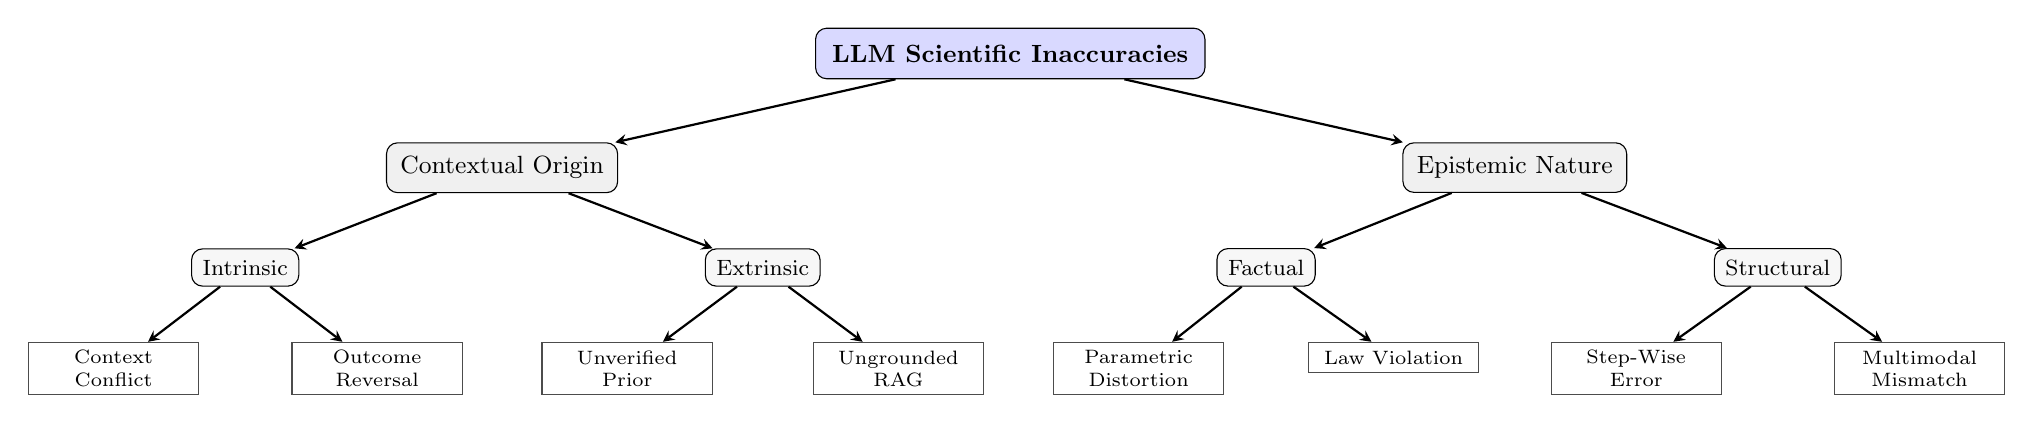
\begin{tikzpicture}[
    node distance=0.8cm and 0.4cm,
    root/.style={rectangle, rounded corners, draw=black, fill=blue!15, font=\bfseries\small, inner sep=6pt},
    axis/.style={rectangle, rounded corners, draw=black, fill=gray!12, font=\small, inner sep=5pt},
    cat/.style={rectangle, rounded corners, draw=black, fill=gray!6, font=\footnotesize, inner sep=4pt},
    leaf/.style={rectangle, draw=black!70, fill=white, font=\scriptsize, align=center, inner sep=3pt, text width=1.95cm},
    arrow/.style={->, >=stealth, thick}
]
\node[root] (root) {LLM Scientific Inaccuracies};
\node[axis, below left=0.8cm and 2.5cm of root] (ctx) {Contextual Origin};
\node[axis, below right=0.8cm and 2.5cm of root] (epi) {Epistemic Nature};

\node[cat, below left=0.7cm and 1.1cm of ctx] (int) {Intrinsic};
\node[cat, below right=0.7cm and 1.1cm of ctx] (ext) {Extrinsic};
\node[cat, below left=0.7cm and 1.1cm of epi] (fac) {Factual};
\node[cat, below right=0.7cm and 1.1cm of epi] (str) {Structural};

\node[leaf, below left=0.7cm and -0.1cm of int] (l1) {Context Conflict};
\node[leaf, below right=0.7cm and -0.1cm of int] (l2) {Outcome Reversal};
\node[leaf, below left=0.7cm and -0.1cm of ext] (l3) {Unverified Prior};
\node[leaf, below right=0.7cm and -0.1cm of ext] (l4) {Ungrounded RAG};
\node[leaf, below left=0.7cm and -0.1cm of fac] (l5) {Parametric Distortion};
\node[leaf, below right=0.7cm and -0.1cm of fac] (l6) {Law Violation};
\node[leaf, below left=0.7cm and -0.1cm of str] (l7) {Step-Wise Error};
\node[leaf, below right=0.7cm and -0.1cm of str] (l8) {Multimodal Mismatch};

\draw[arrow] (root) -- (ctx);
\draw[arrow] (root) -- (epi);
\draw[arrow] (ctx) -- (int);
\draw[arrow] (ctx) -- (ext);
\draw[arrow] (epi) -- (fac);
\draw[arrow] (epi) -- (str);
\draw[arrow] (int) -- (l1);
\draw[arrow] (int) -- (l2);
\draw[arrow] (ext) -- (l3);
\draw[arrow] (ext) -- (l4);
\draw[arrow] (fac) -- (l5);
\draw[arrow] (fac) -- (l6);
\draw[arrow] (str) -- (l7);
\draw[arrow] (str) -- (l8);
\end{tikzpicture}%
}
\caption{Hierarchical taxonomy of language model inaccuracies and hallucination modalities across natural science disciplines (see Section 3).}
\label{fig:taxonomy}
\end{figure*}

\section{Survey Protocol and Methodology}
To maintain rigorous survey standards, our literature synthesis is organized around systematic review criteria. We audited scholarly literature from primary indices, including IEEE Xplore, ACM Digital Library, PubMed, NeurIPS/CVPR/ICLR proceedings, and arXiv preprints published up to 2026.

\subsection{Inclusion and Exclusion Criteria}
Studies were incorporated if they met the following criteria:
\begin{itemize}
    \item They directly propose, evaluate, or benchmark factual accuracy, hallucination detection, or truthfulness metrics in LLMs or Vision-Language Models (VLMs).
    \item They encompass empirical applications across the natural sciences (physics, chemistry, materials science) or biomedical/clinical reasoning.
    \item They introduce formal diagnostic datasets, quantitative metrics, or mechanistic evaluation architectures.
\end{itemize}
We excluded papers that focused exclusively on open-domain creative generation without explicit factuality bounds, unvalidated opinion articles, and duplicate preprints.

\section{Taxonomy and Mechanics of Scientific Hallucination}
As illustrated in Figure~\ref{fig:taxonomy}, hallucinations in scientific applications must be categorized across two orthogonal operational axes: contextual origin and epistemic nature \cite{huang2023survey}.

\subsection{Contextual Origin: Intrinsic vs. Extrinsic}
\textbf{Intrinsic Hallucinations:} An intrinsic hallucination occurs when an LLM's generated assertion directly contradicts reference context explicitly provided in the user prompt \cite{rawte2023survey}. For example, in automated clinical trial summarization, if the context indicates a treatment group outcome of $p=0.04$ and the model states the intervention lacked statistical significance ($p>0.05$), the generation constitutes an intrinsic hallucination.

\textbf{Extrinsic Hallucinations:} An extrinsic hallucination occurs when the model introduces factual statements that can neither be confirmed nor refuted based on the prompt's provided background \cite{huang2023survey}. In open-domain literature synthesis, introducing ungrounded auxiliary hypotheses creates significant risk for downstream empirical validation.

\subsection{Semantic and Epistemic Nature}
\textbf{Factual Hallucinations:} Factual hallucinations arise when an output directly violates established consensus, physical laws, or empirical data stored in real-world knowledge graphs \cite{huang2023survey}. These errors bifurcate into:
\begin{itemize}
    \item \textbf{Intrinsic Factuality Violations:} Flaws in the model's static parametric weights formed during pre-training.
    \item \textbf{Extrinsic Factuality Violations:} Failure to retrieve or ground reasoning within external context retrieved via Retrieval-Augmented Generation (RAG).
\end{itemize}

\textbf{Structural and Logical Hallucinations:} These include non-sequiturs, mathematical reasoning breakdowns across intermediate steps, and semantic self-contradictions within the generated text.

\subsection{Etiology and Mathematical Mechanics}
Hallucinations in scientific models stem from several foundational causes:
\begin{enumerate}
    \item \textbf{Uncurated Pre-training Corpora:} Training on corpora containing outdated scientific assumptions embeds falsehoods directly into model weights \cite{lin2022truthfulqa}.
    \item \textbf{Source-Reference Divergence:} If training pairs associate abstract concepts with unsupported reference claims, the objective teaches the model to extrapolate beyond the supplied premises \cite{huang2023survey}.
    \item \textbf{Probabilistic Decoding Dynamics:} Autoregressive decoding algorithms (e.g., nucleus sampling with temperature $\tau>0$) trade off factual determinism in favor of lexical entropy \cite{rawte2023survey}:
    \begin{equation}
    p(x_{t}=w_{i}\mid x_{<t}) = \frac{\exp(z_{i}/\tau)}{\sum_{j}\exp(z_{j}/\tau)}.
    \end{equation}
    At higher values of $\tau$, the model samples from the distribution tail, increasing the probability of hallucinatory tokens.
\end{enumerate}

\begin{figure}[t]
\centering
\resizebox{\columnwidth}{!}{%
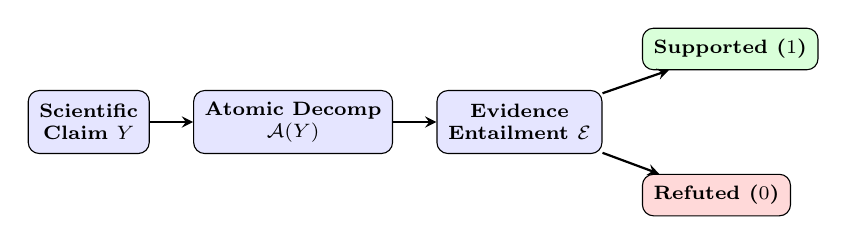
\begin{tikzpicture}[
    node distance=0.55cm,
    box/.style={rectangle, rounded corners, draw=black, fill=blue!10, font=\scriptsize\bfseries, align=center, inner sep=4pt, minimum height=0.8cm},
    outbox/.style={rectangle, rounded corners, draw=black, font=\scriptsize\bfseries, align=center, inner sep=4pt},
    arrow/.style={->, >=stealth, thick}
]
\node[box] (claim) {Scientific\\Claim $Y$};
\node[box, right=of claim] (decomp) {Atomic Decomp\\$\mathcal{A}(Y)$};
\node[box, right=of decomp] (entail) {Evidence\\Entailment $\mathcal{E}$};
\node[outbox, fill=green!15, above right=0.25cm and 0.5cm of entail] (sup) {Supported ($1$)};
\node[outbox, fill=red!15, below right=0.25cm and 0.5cm of entail] (ref) {Refuted ($0$)};

\draw[arrow] (claim) -- (decomp);
\draw[arrow] (decomp) -- (entail);
\draw[arrow] (entail) -- (sup);
\draw[arrow] (entail) -- (ref);
\end{tikzpicture}%
}
\caption{End-to-end operational architecture of an automated atomic-fact verification pipeline (e.g., FActScore \cite{min2023factscore}).}
\label{fig:factscore}
\end{figure}

\section{Literature Review: Domain-Specific Scientific Benchmarks}
Evaluating scientific truthfulness requires measuring spatial reasoning, adherence to physical constants, multi-step calculation, and complex synthesis across conflicting literature.

\subsection{General Sciences, Physics, and Mathematics}
\textbf{SciEval and Bloom's Taxonomy:} Sun et al. \cite{sun2024scieval} introduced SciEval, comprising roughly 18,000 multi-disciplinary questions across chemistry, physics, and biology. Derived from Bloom's Taxonomy, SciEval assesses four progressive cognitive levels: basic recall, applied domain knowledge, scientific calculation, and research-level synthesis. SciEval addresses static data contamination through dynamically generated numerical subsets. Although GPT-4 achieves 73.93\% on static questions, its performance declines on dynamic physics calculations, demonstrating the gap between memorization and symbolic reasoning \cite{sun2024scieval}.

\textbf{GPQA and Scalable Oversight:} Rein et al. \cite{rein2023gpqa} developed GPQA, comprising 448 multiple-choice questions written and validated by domain experts holding or pursuing PhDs in biology, chemistry, and physics. These questions are intentionally ``Google-proof''. Non-expert validators with PhDs in unrelated domains spent over 30 minutes per question with unrestricted internet access, achieving only 34\% accuracy. By contrast, domain experts achieved 65\% accuracy, while baseline GPT-4 attained 39\% \cite{rein2023gpqa}. GPQA establishes an empirical testbed for scalable oversight: supervising systems whose cognitive outputs surpass the verification capacity of human non-experts.

\textbf{SciBench:} Wang et al. \cite{wang2024scibench} created SciBench, featuring 695 college-level textbook problems requiring multi-step calculus, thermodynamics, and quantum mechanical derivations. Models frequently fail along intermediate mathematical trajectories, underscoring the brittleness of purely statistical token prediction in formal mathematics.

\subsection{Biomedical and Clinical Systems}
\textbf{Med-PaLM and Clinical Question-Answering:} Benchmark evaluation in clinical medicine centers on datasets such as MedQA \cite{jin2021disease} (USMLE-style vignettes) and PubMedQA \cite{jin2019pubmedqa}. Singhal et al. \cite{singhal2023large} introduced Med-PaLM, the first model to surpass the USMLE passing threshold (67.2\%). Its successor, Med-PaLM 2 \cite{singhal2023towards}, achieved 86.5\% on MedQA through ensemble refinement and retrieval-augmented reasoning. Physician raters favored Med-PaLM 2 long-form answers over human clinician responses across 8 of 9 operational axes, including factual consensus alignment (preferred 72.9\% of the time) \cite{singhal2023towards}.

\textbf{Adversarial Hallucination Testing via Med-HALT:} Umapathi et al. \cite{umapathi2023medhalt} developed Med-HALT (Medical Domain Hallucination Test) to evaluate hallucination triggers. By introducing contradictory medical premises, Med-HALT measures the frequency of false confirmations, providing an auditing protocol prior to clinical integration.

\subsection{Chemistry, Molecular Graphs, and Multimodality}
\textbf{ChemBench:} Jablonka et al. \cite{jablonka2024superhuman} introduced ChemBench, comprising 2,700 question-answer pairs spanning stoichiometry, thermodynamics, and synthesis design. For quantitative answers, ChemBench requires numeric predictions to fall within a 1\% Mean Absolute Error (MAE) threshold. While state-of-the-art models achieved parity with professional chemists on macro scores, their failure modes revealed severe overconfidence and basic errors in rudimentary tasks like ring counting and stoichiometric balancing \cite{jablonka2024superhuman}.

\textbf{Multimodal Frontiers with MACBENCH:} Scientific literature relies on multimodal data representations, including nuclear magnetic resonance (NMR) spectra, crystal diffraction patterns, and electron microscopy. The MACBENCH framework \cite{anonymous2024macbench} evaluates Vision-Language Models (VLMs) on physical chemistry figures, exposing high rates of visual hallucination when deducing laboratory safety hazards or identifying crystal structures.

\section{Evolution of Factuality Evaluation Methodologies}
The metrics used to quantify factual precision in natural language systems have shifted significantly over time, as shown in Figure~\ref{fig:tradeoff}.

\begin{figure}[t]
\centering
\resizebox{\columnwidth}{!}{%
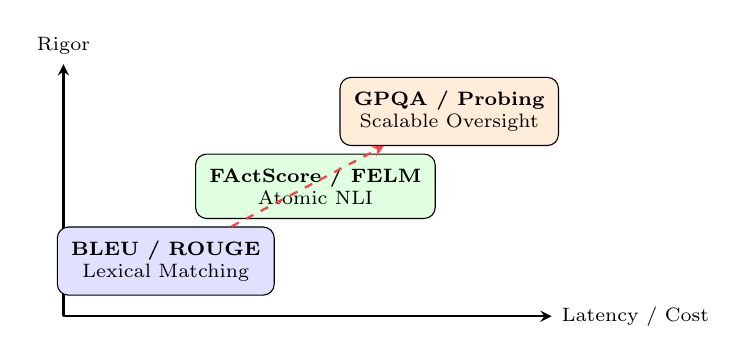
\begin{tikzpicture}[
    node distance=0.8cm,
    stage/.style={rectangle, rounded corners, draw=black, font=\scriptsize\bfseries, align=center, inner sep=5pt},
    arrow/.style={->, >=stealth, thick}
]
\draw[arrow] (0,0) -- (6.2,0) node[right, font=\scriptsize] {Latency / Cost};
\draw[arrow] (0,0) -- (0,3.2) node[above, font=\scriptsize] {Rigor};

\node[stage, fill=blue!12] (s1) at (1.3, 0.7) {BLEU / ROUGE\\{\normalfont\scriptsize Lexical Matching}};
\node[stage, fill=green!12] (s2) at (3.2, 1.65) {FActScore / FELM\\{\normalfont\scriptsize Atomic NLI}};
\node[stage, fill=orange!15] (s3) at (4.9, 2.6) {GPQA / Probing\\{\normalfont\scriptsize Scalable Oversight}};

\draw[->, >=stealth, dashed, red!75, thick] (s1) -- (s3);
\end{tikzpicture}%
}
\caption{Deployment trade-off space comparing factuality evaluation frameworks across verification latency and epistemic rigor.}
\label{fig:tradeoff}
\end{figure}

\subsection{Limitations of Lexical Overlap}
Natural language generation historically relied on $n$-gram overlap metrics:
\begin{equation}
\text{BLEU} = BP \cdot \exp\left(\sum_{n=1}^{N} w_{n}\ln p_{n}\right),
\end{equation}
and ROUGE-L (based on Longest Common Subsequences) \cite{lin2004rouge,papineni2002bleu}. These metrics are unsuited for scientific verification: an LLM can achieve high lexical overlap while completely inverting scientific meaning through a single incorrect token or misplaced negation.

\subsection{Fine-Grained Atomic Decomposition: FActScore}
To address long-form scientific generation, Min et al. \cite{min2023factscore} formulated FActScore. Given a model output $Y$, an extraction operator $\mathcal{A}$ decomposes the text into a set of discrete, atomic claims:
\begin{equation}
\mathcal{A}(Y) = \{c_{1}, c_{2}, \dots, c_{k}\}.
\end{equation}
Each atomic proposition $c_{i}$ is evaluated against an authoritative knowledge base $\mathcal{K}$ through an entailment function $\mathcal{E}(c_{i},\mathcal{K})\in\{0,1\}$. The aggregate FActScore metric is computed as:
\begin{equation}
\text{FActScore}(Y,\mathcal{K}) = \frac{1}{|\mathcal{A}(Y)|}\sum_{i=1}^{|\mathcal{A}(Y)|}\mathcal{E}(c_{i},\mathcal{K}).
\end{equation}
This operational pipeline is illustrated in Figure~\ref{fig:factscore}. On long-form generation, models such as ChatGPT achieved only 58\% atomic precision despite maintaining fluent text generation \cite{min2023factscore}.

\subsection{Classifier and Representation-Space Probing}
Recent developments utilize Natural Language Inference (NLI) classifiers to compute semantic entailment scores over scientific propositions \cite{chen2023felm}. Concurrently, mechanistic interpretability approaches analyze the geometric representations inside LLM activation streams. Techniques such as Contrastive Activation Addition (CAA) \cite{rimsky2023steering} map truthfulness activation vectors in the residual stream, allowing internal hallucination detection prior to token emission.

\subsection{Inverse Scaling Dynamics}
Lin et al. \cite{lin2022truthfulqa} documented the phenomenon of inverse scaling on TruthfulQA. When evaluating model families across scale, larger models (e.g., GPT-3 175B) were systematically less truthful than smaller variants on questions targeted at common human misconceptions. Larger architectures more effectively capture human web misconceptions present in pre-training data, producing imitative falsehoods \cite{lin2022truthfulqa}. Scaling parameter capacity alone is insufficient to guarantee scientific factuality.

\section{Comparative Analysis of Models and Datasets}
A systematic comparison of representative architectures and diagnostic benchmarks is summarized in Table~\ref{tab:models} and Table~\ref{tab:benchmarks}.

\begin{table}[t]
\centering
\caption{Comparative taxonomy of representative state-of-the-art architectures and their characteristic scientific failure modes.}
\label{tab:models}
\footnotesize
\begin{tabularx}{\columnwidth}{>{\raggedright\arraybackslash}p{2.1cm} >{\raggedright\arraybackslash}p{2.1cm} >{\raggedright\arraybackslash}X}
\toprule
\textbf{Model Family} & \textbf{Core Mechanism} & \textbf{Primary Bottlenecks} \\
\midrule
GPT-4 / 4o \cite{openai2024gpt4} & Dense Autoregressive & Context-neglect in long derivations \\
Med-PaLM 2 \cite{singhal2023towards} & Clinical Tuning with ER & High test-time ensemble latency \\
Claude 3.5 Sonnet \cite{anthropic2024claude} & Constitutional Transformer & Multi-truth ambiguity breakdown \\
ChemLLM \cite{zhang2024chemllm} & Molecular Token Adapted & Failure on unseen dynamic topologies \\
o1 / o3-mini \cite{openai2024reasoning} & Test-Time Search & Latent reasoning path hallucination \\
\bottomrule
\end{tabularx}
\end{table}

\begin{table}[t]
\centering
\caption{Systematic landscape of core scientific factuality and reasoning benchmarks.}
\label{tab:benchmarks}
\footnotesize
\begin{tabularx}{\columnwidth}{>{\raggedright\arraybackslash}p{1.85cm} >{\raggedright\arraybackslash}p{1.3cm} >{\raggedright\arraybackslash}X >{\raggedright\arraybackslash}p{1.55cm}}
\toprule
\textbf{Benchmark} & \textbf{Modality} & \textbf{Target Domain} & \textbf{Metric} \\
\midrule
GPQA \cite{rein2023gpqa} & Text & Physics, Chem., Bio (PhD) & Accuracy (\%) \\
SciEval \cite{sun2024scieval} & Text & Multi-level General Science & Bloom's Acc (\%) \\
ChemBench \cite{jablonka2024superhuman} & Text/Num & Physical \& Inorganic Chemistry & $\text{MAE} < 1\%$ \\
PubMedQA \cite{jin2019pubmedqa} & Text & Biomedical Literature & Reasoning $F_1$ \\
Med-HALT \cite{umapathi2023medhalt} & Text & Clinical Medical Reasoning & Hallucination Res. \\
MACBENCH \cite{anonymous2024macbench} & Multimodal & Chemistry \& Materials Science & Grounded VQA \\
TruthfulQA \cite{lin2022truthfulqa} & Text & Scientific \& General Fallacies & \% Truthful \\
\bottomrule
\end{tabularx}
\end{table}

\subsection{Architectural Paradigms}
Table~\ref{tab:models} highlights the tradeoffs across foundation models. Models utilizing test-time search (e.g., OpenAI o1/o3-mini) exhibit stronger logical coherence on multi-step mathematical derivations. However, fine-tuned biomedical architectures like Med-PaLM 2 require structured ensemble refinement to prevent context neglect \cite{singhal2023towards}.

\subsection{Benchmark Landscape}
As detailed in Table~\ref{tab:benchmarks}, benchmarks vary significantly across evaluation stringency. While static question-answering benchmarks (e.g., PubMedQA) are vulnerable to data leakage, dynamic datasets like SciEval and ChemBench test operational understanding by modifying stoichiometric balances and physical boundary conditions programmatically \cite{jablonka2024superhuman,sun2024scieval}.

\section{Open Challenges and Future Directions}
Despite the advances highlighted in Section 4 and Section 5, benchmarking scientific factuality faces four fundamental bottlenecks:

\subsection{Data Contamination and Benchmark Memorization}
Proprietary models scrape massive web corpora that often include public evaluation suites \cite{sun2024scieval}. When static benchmarks leak into training corpora, models recall answers rather than performing genuine scientific inference. Developing procedurally synthesized benchmarks that dynamically generate scientific problems at inference time is a crucial priority.

\subsection{Context Neglect in Retrieval-Augmented Pipelines}
Although RAG provides verified external literature, models frequently display context neglect, defaulting to flawed internal parametric priors. Resolving multi-hop logical deductions across dense academic references remains a difficult problem \cite{shami2026benchmarking}.

\subsection{Multi-Truth Scenarios and Citation Integrity}
Scientific research often involves open debates where multiple valid hypotheses coexist. Current LLMs frequently collapse nuance into singular declarations \cite{patel2024factuality}. Moreover, when prompted to cite evidence, models often produce hallucinated digital object identifiers (DOIs) or misattribute experimental findings \cite{patel2024factuality}.

\subsection{Vision-Language Multimodal Hallucinations}
The shift toward multimodal architectures (e.g., MACBENCH) introduces novel failure modes, such as misinterpreting microscopy artifacts, mistaking spatial orientations in structural biology, or hallucinating features in NMR spectra \cite{anonymous2024macbench}. Future benchmarks must systematically audit cross-modal grounding.

\section{Conclusion}
Benchmarking the factual accuracy of Large Language Models across the natural sciences remains a central challenge in artificial intelligence. As foundation models assume greater responsibility in clinical medicine, materials design, and mathematical derivation, statistical fluency without empirical grounding introduces serious risks. This survey categorized hallucination taxonomies, reviewed specialized benchmarks across scientific disciplines, and traced the shift from lexical overlap metrics to fine-grained atomic claim evaluation and internal representation probing. Mitigating scientific hallucination will require moving beyond static test suites toward dynamic procedural benchmarks, robust scalable oversight frameworks, and autonomous, self-verifying scientific agents.

\bibliographystyle{plainurl}
\bibliography{references}

\end{document}